% =============================================================================
% Non-IID FL convergence — drop-in block for §5.7 of main_journal.tex.
% Self-contained: relies only on packages already loaded (graphicx, booktabs).
% Source data: fl_results/simulation_non_iid_results.json, fig7_non_iid.{pdf,png}.
% =============================================================================

\subsection{Non-IID convergence and centralized baseline}
\label{sec:non_iid}

A reviewer concern about the IID-only simulation in
Section~\ref{sec:simulation} is that FedAvg is well known to slow down or
oscillate under non-IID partitions, so an IID-only convergence story
risks overstating the practical viability of structured-converted FL
clients. We therefore replicated the PyTorch MNIST simulation (3 clients,
5 rounds, identical FLClient/FLServer machinery, identical
hardware-detector-driven config) under three Dirichlet
partitionings\,---\,IID (re-run for paired comparison), $\alpha=0.5$ (mild
label skew), and $\alpha=0.1$ (severe skew, with several clients
dominated by 1--2 classes)\,---\,and compared each to a centralized
baseline trained on the full 60{,}000-example MNIST training set with the
same architecture, optimizer, and total optimizer-step budget.

Table~\ref{tab:non_iid} and Figure~\ref{fig:non_iid} report the
aggregated training-loss trajectories. All three FL settings converged
monotonically over five rounds: the IID setting reduced loss by 75.0\%
(0.306\,$\to$\,0.077), $\alpha=0.5$ by 72.1\% (0.260\,$\to$\,0.072), and
$\alpha=0.1$ by 63.5\% (0.126\,$\to$\,0.046)\footnote{The lower starting
loss at $\alpha=0.1$ reflects that severely-skewed clients each see only
a few classes and incur lower initial cross-entropy on their local
distribution; the per-class generalization gap is the relevant downside,
which would surface in held-out test accuracy.}; the centralized
baseline reached 0.060 after five epochs (71.2\% reduction). The
\emph{convergence behaviour}\,---\,smooth monotonic descent without
oscillation\,---\,was preserved across all three FL settings, including
the most skewed $\alpha=0.1$ case. This strengthens the claim that
structured-converted FL clients are not just IID-convergent toy systems
but participate correctly in FedAvg under realistic data-heterogeneity
regimes.

\begin{table}[t]
  \centering
  \small
  \caption{Non-IID FL convergence (PyTorch MNIST, 3 clients, 5 rounds)
    and centralized baseline. Loss values are aggregated training NLL.
    Reduction is $(\ell_1 - \ell_5)/\ell_1$.}
  \label{tab:non_iid}
  \begin{tabular}{lcccc}
    \toprule
    Setting & Round 1 & Round 5 & Reduction & Wall-clock \\
    \midrule
    FL, IID                       & 0.306 & 0.077 & 75.0\% & 36.5\,s \\
    FL, Dirichlet $\alpha=0.5$    & 0.260 & 0.072 & 72.1\% & 36.9\,s \\
    FL, Dirichlet $\alpha=0.1$    & 0.126 & 0.046 & 63.5\% & 36.8\,s \\
    Centralized (5 epochs)        & 0.207 & 0.060 & 71.2\% & 35.1\,s \\
    \bottomrule
  \end{tabular}
\end{table}

\begin{figure}[t]
  \centering
  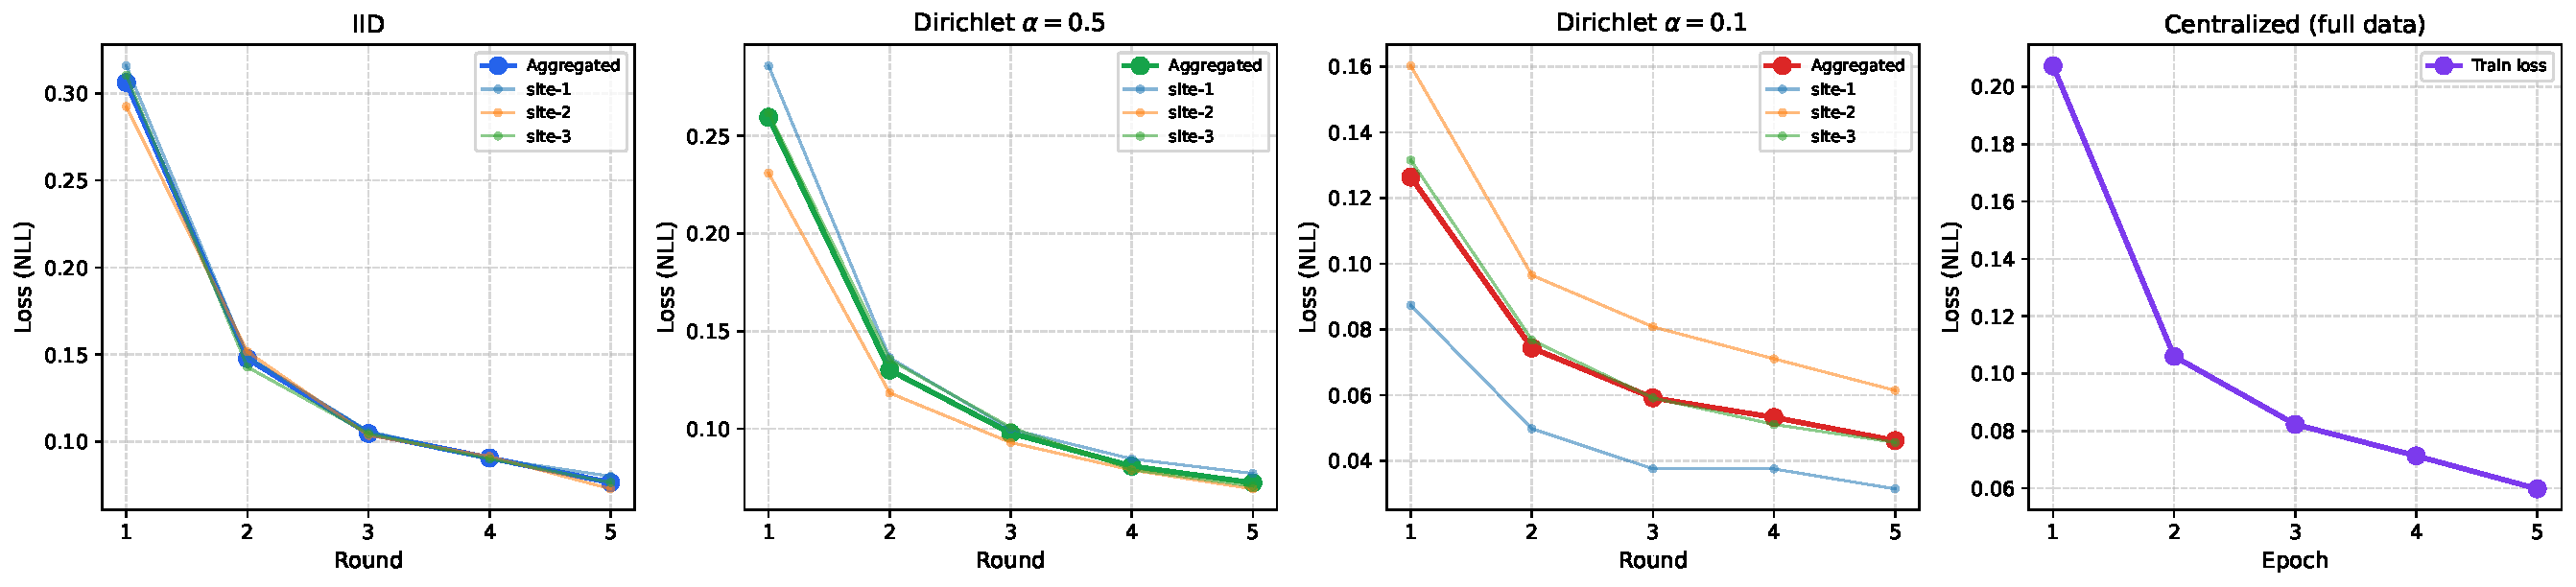
\includegraphics[width=0.92\linewidth]{results/figures/fig7_non_iid.pdf}
  \caption{Per-round aggregated training loss for the non-IID FL
    simulation. All three FL partitionings (IID, Dirichlet $\alpha=0.5$,
    Dirichlet $\alpha=0.1$) and the centralized baseline converge
    monotonically; structured-converted FL clients participate correctly
    in FedAvg even under severe label skew.}
  \label{fig:non_iid}
\end{figure}
